\section{510 --- Inorder Successor in BST II}
Given a binary search tree and a node in it, find the in-order successor of that node in the BST.

The successor of a node $p$ is the node with the smallest key greater than the value of $p$.

You will have direct access to the node but not to the root of the tree. Each node will have a reference to its parent node.
 

\paragraph{Example 1:}

\begin{flushleft}

\textbf{Input}:

\begin{figure}[H]
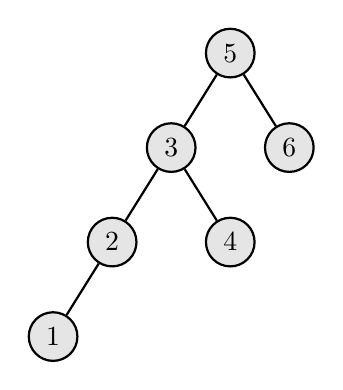
\begin{tikzpicture}
[every node/.style={draw, circle,minimum size=6mm, fill=gray!20!},
  level distance=12mm,  thick]
\node{5}
  child{node{3} child{node{2} child{node{1}} child[missing]} child{node{4}}}
  child{node{6}};
\end{tikzpicture}
\end{figure}
 
$ p = 1 $

\textbf{Output}: 2

\textbf{Explanation}: 

1's in-order successor node is 2. Note that both $p$ and the return value is of Node type.
\end{flushleft}

\paragraph{Example 2:}

\begin{flushleft}
\textbf{Input}: 
\begin{figure}[H]
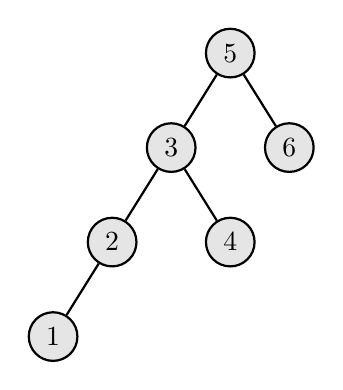
\begin{tikzpicture}
[every node/.style={draw, circle,minimum size=6mm, fill=gray!20!},
  level distance=12mm,  thick]
\node{5}
  child{node{3} child{node{2} child{node{1}} child[missing]} child{node{4}}}
  child{node{6}};
\end{tikzpicture}
\end{figure}
$ p = 6 $

\textbf{Output}: $\emptyset$

\textbf{Explanation}: 

There is no in-order successor of the current node, so the answer is $\emptyset$.
\end{flushleft}

\paragraph{Example 3:}

\begin{flushleft}

\textbf{Input}:
\begin{figure}[H]
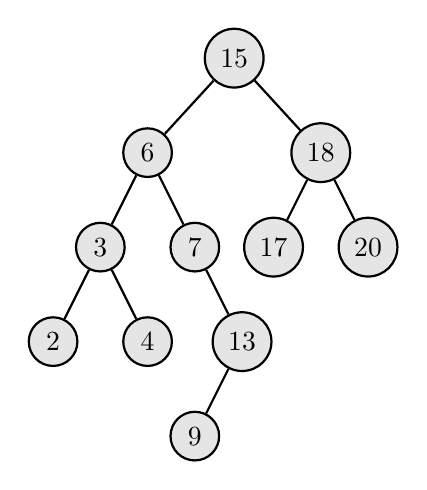
\begin{tikzpicture}
[every node/.style={draw, circle,minimum size=6mm, fill=gray!20!},
  level distance=12mm,  thick, level 1/.style={sibling distance=22mm}, level 2/.style={sibling distance=12mm}]
\node{15}
  child{node{6} child{node{3} child{node{2}} child{node{4}}} child{node{7} child[missing] child{node{13} child{node{9}} child[missing]}}}
  child{node{18} child{node{17}} child{node{20}}};
\end{tikzpicture}
\end{figure}
 
$ p = 15 $


\textbf{Output}: 17

\end{flushleft}

\paragraph{Example 4:}

\begin{flushleft}

\textbf{Input}: 
\begin{figure}[H]
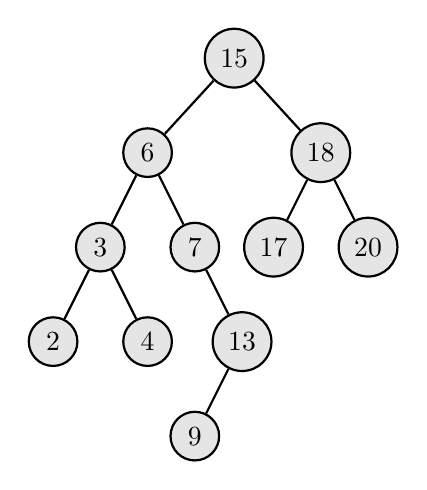
\begin{tikzpicture}
[every node/.style={draw, circle,minimum size=6mm, fill=gray!20!},
  level distance=12mm,  thick, level 1/.style={sibling distance=22mm}, level 2/.style={sibling distance=12mm}]
\node{15}
  child{node{6} child{node{3} child{node{2}} child{node{4}}} child{node{7} child[missing] child{node{13} child{node{9}} child[missing]}}}
  child{node{18} child{node{17}} child{node{20}}};
\end{tikzpicture}
\end{figure}

$ p = 13 $

\textbf{Output}: 15
\end{flushleft}
 

\paragraph{Note:}

\begin{itemize}
\item If the given node has no in-order successor in the tree, return $\emptyset$.
\item It's guaranteed that the values of the tree are unique.
\item Remember that we are using the \textbf{Node} type instead of \textbf{TreeNode} type so their string representation are different.
\end{itemize} 

\paragraph{Follow up:}

\begin{itemize}
\item Could you solve it without looking up any of the node's values?
\end{itemize}

\subsection{Iteration}
在BST中,一个node在inorder traverse的successor node取决于该node是否有right child

\begin{itemize}
\item Has a \textbf{right} child: the successor node is somewhere lower in the tree. To find the successor, go to the right once and then go left always.

For example: The following binary tree's inorder traverse sequence is 1, 2, 7, 11, 12, 13, 25, 33, 34, 36, 40. The node 33' successor is 34.
\begin{figure}[H]
\begin{tikzpicture}
[every node/.style={draw, circle,minimum size=6mm, fill=gray!20!},node distance=8mm, thick]
\node{2}
child{node{1}}
child{node[fill=red!20!](a){33} 
		child{node{25} child{node{11} child{node{7}} child{node{12} child[missing] child{node{13}}} } child[missing]} 
		child{node{40} child{node(b)[fill=blue!20!]{34} child[missing] child{node{36}}} child[missing]}
	};
\node[single arrow, rotate=195, minimum height=1.5cm, fill=red!20!](r1) at ($(a.north east) + (1.2,0.2)$) {};
\node[draw=none,fill=none, rotate=10] at ($(r1.west) + (0.5,0.1)$) {\small node};
\node[single arrow, rotate=165, minimum height=1.5cm, fill=blue!20!](r2) at($(b.east) + (1.2,-0.2)$) {};
\node[draw=none,fill=none, rotate=-12] at ($(r2.west) + (0.8,-0.2)$) {\small succesor};
\end{tikzpicture}
\caption{Successor of the node with a right child: one step right and then left till you can.}
\end{figure}
\item No right child: the successor is somewhere upper in the tree. To find the successor, go up till the node that is left child of its parent. The answer is the parent. Beware that there could be no successor in such a situation.

\begin{figure}[H]
\begin{tikzpicture}
[every node/.style={draw, circle,minimum size=6mm, fill=gray!20!},node distance=8mm, thick]
\node{2}
child{node{1}}
child{node{33} 
		child{node(b)[fill=blue!20!]{25} child{node(p2){11} child{node{7}} child{node(p1){12} child[missing] child{node[fill=red!20!](a){13}}} } child[missing]} 
		child{node{40} child{node{34} child[missing] child{node{36}}} child[missing]}
	};
\node[single arrow, rotate=195, minimum height=1.5cm, fill=red!20!](r1) at ($(a.north east) + (1.2,0.2)$) {};
\node[draw=none,fill=none, rotate=10] at ($(r1.west) + (0.5,0.1)$) {\small node};
\node[single arrow, rotate=15, minimum height=1.5cm, fill=blue!20!](r2) at($(b.west) + (-1.2,-0.2)$) {};
\node[draw=none,fill=none, rotate=12] at ($(r2.west) + (-0.8,-0.2)$) {\small succesor};
\path (a)--(p1)coordinate[at start](h1)coordinate[at end](h2);
\draw[red, >=stealth, ->] ($(h1)!-6pt!90:(h2)$)--($(h2)!-6pt!-90:(h1)$);
\path (p1)--(p2)coordinate[at start](h3)coordinate[at end](h4);
\draw[red, >=stealth, ->] ($(h3)!-6pt!90:(h4)$)--($(h4)!-6pt!-90:(h3)$);
\path (p2)--(b)coordinate[at start](h5)coordinate[at end](h6);
\draw[red, >=stealth, ->] ($(h5)!-6pt!90:(h6)$)--($(h6)!-6pt!-90:(h5)$);
\end{tikzpicture}
\caption{Successor of the node without right child: Go up till the node that is the \textbf{left} child of its parent, then return the parent}
\end{figure}

The following case is an example of null successor.
\begin{figure}[H]
\begin{tikzpicture}
[every node/.style={draw, circle,minimum size=6mm, fill=gray!20!},node distance=8mm, thick]
\node(p2){2}
child{node{1}}
child{node(p1){33} 
		child{node{25} child{node{11} child{node{7}} child{node{12} child[missing] child{node{13}}} } child[missing]} 
		child{node[fill=red!20!](a){40} child{node{34} child[missing] child{node{36}}} child[missing]}
	};
\node[single arrow, rotate=195, minimum height=1.5cm, fill=red!20!](r1) at ($(a.north east) + (1.2,0.2)$) {};
\node[draw=none,fill=none, rotate=10] at ($(r1.west) + (0.5,0.1)$) {\small node};
\path (a)--(p1)coordinate[at start](h1)coordinate[at end](h2);
\draw[red, >=stealth, ->] ($(h1)!-6pt!90:(h2)$)--($(h2)!-6pt!-90:(h1)$);
\path (p1)--(p2)coordinate[at start](h3)coordinate[at end](h4);
\draw[red, >=stealth, ->] ($(h3)!-6pt!90:(h4)$)--($(h4)!-6pt!-90:(h3)$);
\node[draw=none, fill=none](t) [above = 8mm of p2, xshift=-5mm] {};
\path (p2)--(t)coordinate[at start](h5)coordinate[at end](h6);
\draw[red, >=stealth, ->] ($(h5)!-6pt!90:(h6)$)--($(h6)!-6pt!-90:(h5)$);
\node[single arrow, rotate=15, minimum height=1.5cm, fill=blue!20!](r2) at($(t.west) + (-0.5,-0.4)$) {};
\node[draw=none,fill=none, rotate=12] at ($(r2.west) + (-1.1,-0.2)$) {\small null succesor};
\end{tikzpicture}
\caption{Successor of the node without right child: Go up till the node that is the \textbf{left} child of its parent, then return the parent}
\end{figure}

\end{itemize}


\setcounter{lstlisting}{0}
\begin{lstlisting}[style=customc, caption={Iteration}]
Node* inorderSuccessor( Node* node )
{
    if( node->right )
    {
        //turn right
        //and then go till left down
        auto x = node->right;

        while( x->left )
        {
            x = x->left;
        }

        return x;
    }

    //otherwise,
    //go up until a node
    //is the left node of its parent
    auto x = node;
    while( ( x->parent ) && ( x->parent->right == x ) )
    {
        x = x->parent;
    }

    return x->parent;
}
\end{lstlisting}
